\documentclass[12pt]{article}
%Fonts
\usepackage[utf8]{inputenc}
\usepackage[T1]{fontenc}
%\usepackage{XCharter}
\usepackage{graphicx}
\usepackage{booktabs}
\usepackage[document]{ragged2e}
% Table
\usepackage{tabularx}
\usepackage{multirow}
% URL
\usepackage{hyperref}
\usepackage{enumitem}
%DOCUMENT MARGINS
\usepackage{geometry}
\usepackage{graphicx,wrapfig,lipsum}

\usepackage[framemethod=tikz]{mdframed} % Allows defining custom boxed/framed environments
\usepackage{amsmath}
\geometry{
	paper=a4paper, % Paper size, change to letterpaper for US letter size
	top=2.5cm, % Top margin
	bottom=3cm, % Bottom margin
	left=2.5cm, % Left margin
	right=2.5cm, % Right margin
	headheight=14pt, % Header height
	footskip=1.5cm, % Space from the bottom margin to the baseline of the footer
	headsep=1.2cm, % Space from the top margin to the baseline of the header
	%showframe, % Uncomment to show how the type block is set on the page
}

%	FILE CONTENTS ENVIRONMENT
%----------------------------------------------------------------------------------------

% Usage:
% \begin{file}[optional filename, defaults to "File"]
%	File contents, for example, with a listings environment
% \end{file}

\mdfdefinestyle{file}{
	innertopmargin=1.6\baselineskip,
	innerbottommargin=0.8\baselineskip,
	topline=false, bottomline=false,
	leftline=false, rightline=false,
	leftmargin=2cm,
	rightmargin=2cm,
	singleextra={%
		\draw[fill=black!10!white](P)++(0,-1.2em)rectangle(P-|O);
		\node[anchor=north west]
		at(P-|O){\ttfamily\mdfilename};
		%
		\def\l{3em}
		\draw(O-|P)++(-\l,0)--++(\l,\l)--(P)--(P-|O)--(O)--cycle;
		\draw(O-|P)++(-\l,0)--++(0,\l)--++(\l,0);
	},
	nobreak,
}

% Define a custom environment for file contents
\newenvironment{file}[1][File]{ % Set the default filename to "File"
	\medskip
	\newcommand{\mdfilename}{#1}
	\begin{mdframed}[style=file]
}{
	\end{mdframed}
	\medskip
}

%	COMMAND LINE ENVIRONMENT
%----------------------------------------------------------------------------------------

% Usage:
% \begin{commandline}
%	\begin{verbatim}
%		$ ls
%		
%		Applications	Desktop	...
%	\end{verbatim}
% \end{commandline}

\mdfdefinestyle{commandline}{
	leftmargin=10pt,
	rightmargin=10pt,
	innerleftmargin=15pt,
	middlelinecolor=black!50!white,
	middlelinewidth=2pt,
	frametitlerule=false,
	backgroundcolor=black!5!white,
	frametitle={Command Line},
	frametitlefont={\normalfont\sffamily\color{white}\hspace{-1em}},
	frametitlebackgroundcolor=black!50!white,
	nobreak,
}

% Define a custom environment for command-line snapshots
\newenvironment{commandline}{
	\medskip
	\begin{mdframed}[style=commandline]
}{
	\end{mdframed}
	\medskip
}

%----------------------------------------------------------

%-----------------------------------------------

\setlength{\parindent}{0em}
% ----------------------------------------
\begin{document}
\newgeometry{top=5cm,bottom=0.1cm}
\begin{titlepage}
\begin{center}

    \textbf{\LARGE \vspace*{15pt}Indian Institute of Technology, Kanpur}
\end{center}
\begin{figure}[h]
\centering

\includegraphics[scale=0.7]{images/bluelog.jpg}
\end{figure}
    \begin{center}
    \textbf{\Large CS685A: Data Mining\\
        Project Report \\}
\end{center}


\begin{center}
\vspace{1 cm}
\rule{\textwidth}{2pt}\linebreak
\Large
\textbf{Title: Analysis of number of child births and infant deaths in India}
\rule{\textwidth}{2pt}\\
\vspace{2.5 cm}
\Large
\textbf{Supervised By: Prof. Arnab Bhattacharya}\\
\vspace{2.5cm}
\normalsize{26 November 2020}

\end{center}
\end{titlepage}
\newpage

\restoregeometry
\begin{titlepage}
    \begin{center}
        \begin{center}
        \textbf{\Large Submitted By: Group 5}\\
        \end{center}

        \medskip

        \vspace{1cm}
        \rule{\textwidth}{2pt}
        \large{Lavlesh Mishra \hfill 19111048(lavleshm@iitk.ac.in)}\\
        \large{Kuldeep Kumar Solanki \hfill 19111045(kuldeeps@iitk.ac.in)}\\
        \large{Jaydeep Meda \hfill 19111039 (jaydeepm@iitk.ac.in)}\\
        \large{Aditya Jain \hfill 20111004 (adityaj20@iitk.ac.in)}\\
        \large{Rohit Singh \hfill 20111418 (kun20@iitk.ac.in)}\\
        \medskip
        \rule{\textwidth}{2pt}
    \end{center}
\end{titlepage}
\newpage
\tableofcontents
\newpage
\section{Abstract}
\justifying
To monitor the performance and quality of the health services being provided under the (National Health Mission)NHM, the Ministry of Health & Family Welfare, Government of India, is putting in place several mechanisms that would strengthen the monitoring and evaluation systems, through performance statistics, surveys, community monitoring, quality assurance etc. Government releases the Health Management Information System(HMIS) database in public domain, which we are using along with the census data to analyse the total number of births, still births and infant deaths in a year for a particular district.

\section{Broad Aims of the project}
To create a model that predicts the number of child births and infant deaths in a year for all district of India.

\setlength{\parindent}{0em}

\section{Datasets}
\subsection{Performance of Key Health Management Indicators for each district in India (HMIS)}

This data is released by Ministry of Health under National Health Mission flagship program which seeks to provide effective healthcare to the rural population throughout the country.

\bigskip

Data set includes the key indicators which affects health of mother and child during pregnancy and at the time of delivery. Data also reports the number of children born, number of still-births and number of infant deaths in each district in a particular year.

Data set is available for years 2008 to 2019. Data set is available in the format of Financial years that is from 1st April of a year to the 31st March of the next year.

\bigskip

Link to the data:\\ \url{https://www.nrhm-mis.nic.in/hmisreports/frmstandard_reports.aspx}

\medskip
Route to the data set files:\\
Performance of Key HMIS Indicators(upto District Level)/20XX-20XX/MonthUpToMarch/\\
Select\_State/All.xls/Click here to donwload 


\subsection{Census Data 2001 and 2011}

The Census of India is conducted every 10 years Ministry of Home Affairs. The Census Data is available in public domain. The data is available at district level for total population, age, disability, education, migration, religion, and various other features.\\

Data is available for the years 2001 and 2011. From these two files, we have generated projections of census data for the years 2008 to 2018. 

\medskip

Link to Census 2001:\\ \url{https://censusindia.gov.in/DigitalLibrary/TablesSeries2001.aspx}

\medskip

Link to Census 2011:\\ \url{https://censusindia.gov.in/2011census/population_enumeration.html}

\newpage
% Data Transformation -----------------------------------------------
\section{Data Transformation}
Our training model requires dataset in well structured format. Data we found was in unstructure excel files for both the datasets - Census and HMIS. We need to transform this data into structured csv files. Characterisitics fo these files are as follows:\\
\begin{itemize}
	\item There are 70 files of Census data. In which 35 are xls files for the Census-2001 and 35 xlsx files for the Census-2011.
	\item There are 385 xls files in HMIS data set. There are 11 xls files for each state, each file for a financial year from 2008 to 2019.
\end{itemize}

\subsection{Transformation of HMIS data:}

HMIS data is present in unstructured xls files. The attributes are merged into single cell entry in excel file. Figure 1 shows merged cells of the HMIS data. These files present in excel extension but they are written in XML format and then converted into excel by the Ministry of Health. Since these are actually XML files, we can't process them using xldr library.

\begin{figure}[h]
	\centering
	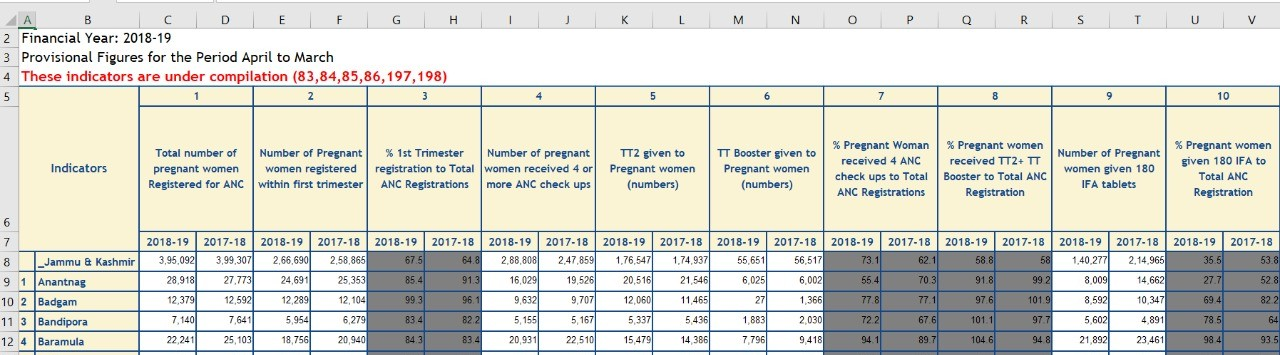
\includegraphics[scale=0.39]{images/hmisfile.jpeg}
	\caption{HMIS data}
\end{figure}

To process them we copied the content from all these 385 files into csv (comma separated) files and then processed these csv files. Steps we followed to transform these XML embedded excel files into structure csv is as follows:
\begin{enumerate}
	\item Download 385 xls files from the HMIS website.
	\item Files downloaded from the website have a default name 'All.xls'. So to process different states and years, we renamed these files as per the state names and year. We used the following command of linux terminal to rename all the file belonging to a state at a time: 
	 
	\begin{commandline}
	\$ for file in *; do mv "$file" "$(basename "\$file")StateName2016-2017"; done;
	\end{commandline} 
	
	We executed the above command 35 times, once for each state.
	
	\item To convert the extension of excel files to csv we used the following command of linux terminal:
	\begin{commandline}
	\$ for i   in *.xlsx; do  libreoffice --headless --convert-to csv "\$i" ; done
	\end{commandline}
	  
\end{enumerate}

After performing above steps we got the files in structured form on which we can perform processing using python libraries.




\subsection{Transformation of Census data:}
Excel files of Census data is semi-structured and to convert them into structured comma separated files (csv), we used \textbf{xlrd} library of python to process it. The xlrd is a library for reading data and formatting information from Excel files, whether they are .xls or .xlsx files.\\


\begin{commandline}
\$ pip3 install xlrd

\medskip
\$ python3 census-transform.py
\end{commandline}

   



% Data Pre-processing -----------------------------------------------
\section{Data Pre-processing}

In this section, we have discussed the pre-processing of the two data set individually, before integrating them into one. We processed following files:

\subsection{Pre-processing of HMIS data:}

\textbf{Characteristics of Data}\\
HMIS data has the following characteristics:
\begin{enumerate}
	\item There are 385 csv files for every 28 States and 7 Union Territories. Telangana and Ladakh are not considered as they are not in Census data.
	\item Data set has 163 attributes.
	\item Each files stores the data for two years and hence there are 325 columns in the csv files.
	\item One attribute is of category type rest all attributes are discrete variables.
\end{enumerate}


\bigskip
\textbf{Cleaning}
\begin{itemize}
	\item Data is redundant in each files as each files contains data for two financial years. We removed the data of one financial year as it was present in the other files.
	\item Many attributes of the data set has missing values, since there was no way to predict these values, we removed such attributes from the dataset.  
\end{itemize}


\subsection{Pre-processing of Census data:}

\textbf{Characteristics of Data}\\
Census data for year 2001 has the following characteristics:
\begin{enumerate}
	\item There are 35 files for every 28 States and 7 Union Territories. Telangana and Ladakh were not created at that time.
	\item Data set has 64 attributes.
	\item One attribute is of category type rest all attributes are discrete variables.
	\item Data is divided on the proximity - Rural and Urban
\end{enumerate}


Census data for year 2011 has the following characteristics:
\begin{enumerate}
	\item There are 35 files for every 28 States and 7 Union Territories. Telangana and Ladakh were not created at that time.
	\item Data set has 94 attributes.
	\item Data is divided on the proximity - Rural and Urban
\end{enumerate}

\bigskip
\textbf{Inconsistency in data}\\
Files contains much inconsistent data:
\begin{itemize}
	\item 'All ages’ attribute includes 'age not stated’, i.e. the attribute - 'All ages' has data for the people whose age are not known.
	\item 'Literate’ attribute includes figures for ‘literates without educational level’ and ‘educational levels not classifiable’.
	\item District IDs are outdated. Since 2011 many districts are newly created which lead to the change of district IDs.	
	\item 'Matric/ secondary but below graduate' includes 'non-technical diploma and certificate not equal to degree'.
	\item Ever married women includes currently married, widowed, divorced and separated.	
	\item There are missing values in the dataset, represented by NaN.
\end{itemize}

\bigskip
\textbf{Cleaning}
\begin{itemize}
	\item We needed statistics for entire district and not in terms of rural and urban regions, so we computed the statistics of entire districts from these two fields.
	\item Many attributes of the data set has missing values, since there was no way to predict these values, we removed such attributes from the dataset.
	\item There are cases where some of the attributes' value is NaN. We handle it by setting these values to zero. Imputing with mean, median or mode was not a suitable choice as there are very less concerned data from which these quantities were to be calculated. The concerened data is the data examples for the same district among all the years. Since there are only 11 years, calculating mean, mode or median is not suitable.
	\item Much of the inconsistencies mentioned above are left in the data. They are handled at outlier analysis stage of the data exploration.  
\end{itemize}


\subsection{Generation of Census data for years 2008 to 2019}
 The Census data was present for the year 2001 and 2011 only but we need the data for each year from 2008 to 2019 to map with the HMIS data. So we have generated the data for the years 2008-2019, using the Compound Interest formula.
\begin{itemize}
\item The Growth Rate(r) is calculated using the 2001 data as Principal(p) and 2011 data as the final amount(p+i). Here i is the Interest.
$$ 
(1+r)^{10} = \frac{Census-2011\enspace stats}{Census-2001 \enspace stats} 
$$

Growth rate r is constant over here, which means the interpolation is geometric and not linear.
\item Data is generated for the remaining years using calculated growth rate(r).
$$
\text{Census Stats for the year Y} =  (1 + r)^{(Y-2001)}
$$
\end{itemize}

Using above method we generated 385 Census files from 70 original files. 11 files for each state, each for one year.

\section{Feature Selection}

\subsection{Feature selection on Census Data}
Features selected from this data are: "NAME", 'TOT\_P','P\_LIT', 'MAINWORK\_P', 'MARGWORK\_P', 'NON\_WORK\_P'. These feautures are renamed to relevant names:
\begin{itemize}
	\item Area Name: It represent the district name.
	\item Population Persons: It represents the total population of the district in that year.
	\item Literate Persons: It represents the total number of literate individuals in the district in that year. Literate persons are the people who have completed at least Matric.
	\item Main workers Persons: It represents the total number of individuals that are involved in any one of the following activities:
	\begin{itemize}
		\item Culitvators
		\item Agricultural labourers
		\item Household Industry workers
		\item Other work
	\end{itemize}
	\item Marginal workers Persons: It represents the total number of individiuals that do marginal work in the district.
	\item Non-workers Persons: It represents the total number of individuals that are unemployed.
\end{itemize}

\subsection{Feature selection on HMIS Data}

Out of 163 attributes we filtered out 42 attributes for our project. There are many attributes which represent the percentage of the other attributes. We dropped such attributes as they can be derived from the other attributes otherwise they would increase the problem of multi-collinearity.\\

There are 8 for which there is no data available so to reduce the strain on missing value treatement step we removed these attributes. There are 6 attributes which contains very low values or the value zero. These discrete values seemed very unrealistic for an entire district, so to reduce the strain on outlier analysis, we removed such attributes from our data set. 


% Data Integration -----------------------------------------------
\section{Data Integration}

We have two data sets - HMIS and Census and we need to merge these two data sets to obtain one single data set one which we can learn a regression model to predict the target variables. So in this section we will discuss the techniques we used to integrate the datasets.\\

Both the datasets has one same attribute. This attribute is 'Area Name' in Census data and it is 'Indicator' in HMIS data. Both represent the name of the district of India. So we performed natural join on this common attribute to obtain the merger of both the data sets.\\

\textbf{Problems in Integrating:}\\
To integrate 385 files of Census and 385 files of HMIS we faced following problems:
\begin{itemize}
	\item District names in both the files are given in different format. In Census data string - "District-" is appended before each of the district's name.
	\item Some district is represented by different names in different data sets.
	\item The name of the districts is changed over the years.
	\item For some of cases the spelling of district names in both the data files do not match.
\end{itemize}

\bigskip
\textbf{Solutions Implemented}\\
We handled above discussed problems using various techniques. We removed the additional strings from the 'Area Name' attribute of the Census data. 

We used Edit-Distance algorithm to map the cases of different spellings. Target distance for the algorithm was set to 3, on increasing the value greater than that was leading to wrong mapping of district names. There were some cases which Edit-Distance can't handle, so we renamed those explicitly by hard code. \\

There were many cases in which there were less districts in Census data in comparision to Census data. So in such cases we were forced to drop the data examples from the HMIS data set to map the data completely.

So after doing all the processing we merged 770 csv files to generate one single csv file - 'all\_states\_merged\_8to18.csv'

\newpage
\section{Data Exploration}

\begin{figure}[h]
	\hspace{-1cm}
	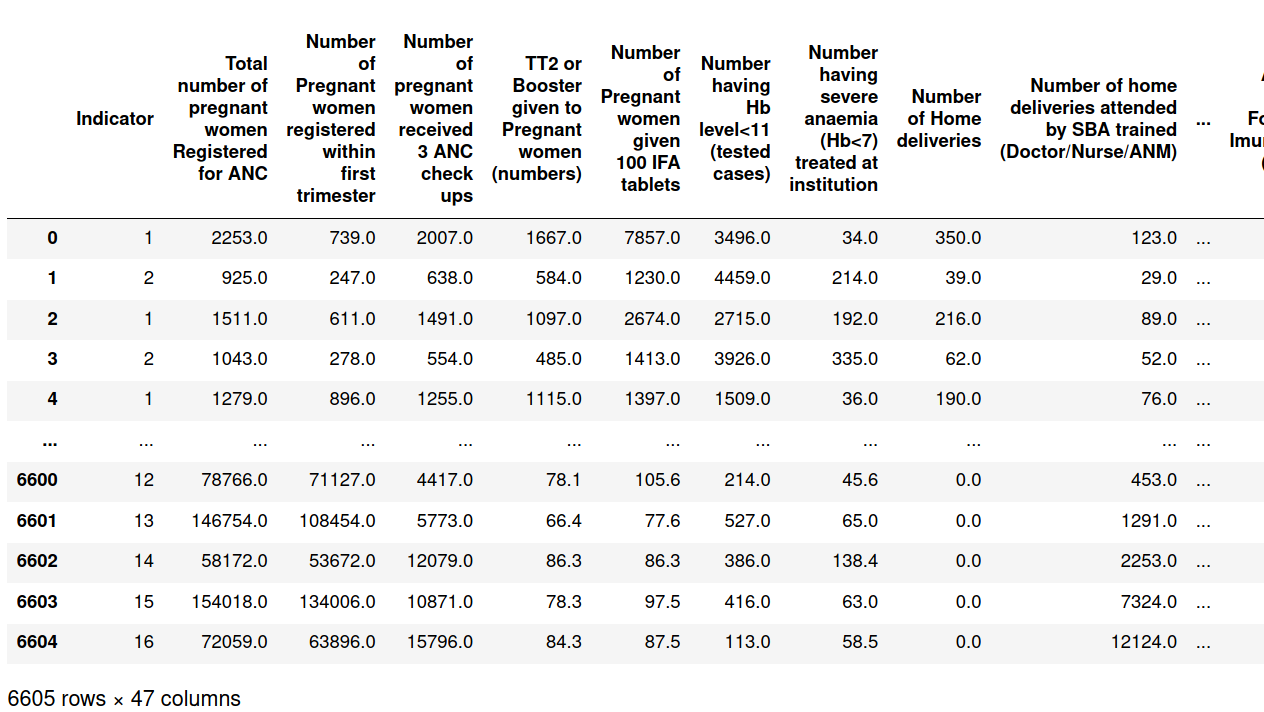
\includegraphics[scale=0.4]{images/data.png}
	\caption{Dataset of Project}
\end{figure}

There are xxx data examples in our data set. Each data example has 47 dimensions.

\subsection{Univariate Analysis}

At this stage, we explore variables one by one. We found that out of \textbf{47 varibles/attributes}, only one attribute 'Indicator' is categorical and all other variables are of type discrete. Out of these 46 discrete variables, 5 variables are of integer data type an rest 41 are of float data type.\\
Since we are solving regression problem, categorical data "Indicator" is of no use in our prediction. So we removed it from the data set.

\subsection{Independent and Dependent variable identification}
We first, identify \textbf{Predictor }(Input) and \textbf{Target }(output) variables. We have three regression problems, so for each problem diffrent independent and dependent variables are needed to found.\\

\textbf{Case 1: Predicting number of Births in a year}\\
Independent$\backslash$Target attribute: 'Total Number of reported live births'\\
Dependent attributes: Rest 45 attributes of the dataset.\\

\textbf{Case 2: Predicting number of Still-Births in a year}\\
Independent$\backslash$Target attribute: 'Total Number of reported Still Births'\\
Dependent attributes: Rest 45 attributes of the dataset.\\

\textbf{Case 3: Predicting number of Infant-Deaths in a year}\\
Independent$\backslash$Target attribute: 'Total Number of reported Infant Deaths'\\
Dependent attributes: Rest 45 attributes of the dataset.\\

\subsection{Multivariate Analysis}

In this section, we found out the relationship between two variables. Here, we looked at the association and disassociation between variables at a pre-defined significance level.

\subsubsection{Collinearity Test}

\begin{figure}[h]
	\centering
	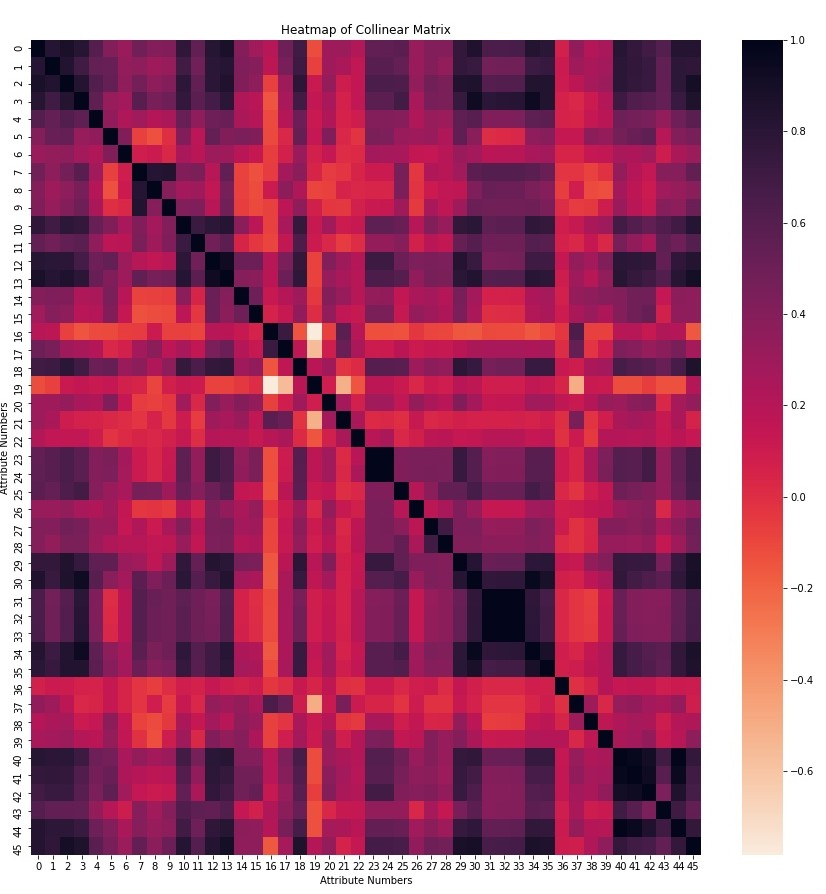
\includegraphics[scale=0.4]{images/heatmap.jpg}
	\caption{Heatmap of Collinear Matrix of dataset}
\end{figure}

There are lot of dark squares in above heat map. So it shows that data attributes are highly correlated to each other.

We found that the attribute 'Number of Pregnant women registered within first trimester' is highly correlated to the attributes - 'Deliveries Conducted at Public Institutions', 'Number of pregnant women received 3 ANC check ups', 'TT2 or Booster given to Pregnant women (numbers)'. This shows that women who registered within first trimester with ANC receives 3 ANC check ups, TT2 supplement are very likely to have delivery at some institution- clinic -public or private. Women those have home deliveries don't register themselves with ANC.

\subsection{Missing Value Treatment}

Missing Value analysis is most tricky part of this data exploration as there are no NaN values in our dataset at this stage. All NaN values in Census data were taken care at the individual pre-processing of the census files, as discussed in the section 5.2 and the one which cannot be taken care was made equal to zero. In HMIS data there are no NaN values but there are values which are equal to zero. \\

The tricky part is whether these zero values are missing values or actual value of the data example is zero. So we can't do anything to our dataset at this stage, but our outlier analysis can find our whether these zero values are genuine or not. Outlier Analysis will mark the NaN values written as zero as outlier and will remove them.

\subsection{Outlier Analysis}

Outlier is an observation that appears far away and diverges from an overall pattern in a sample. In this section, we will discuss two outlier detection techniques that we applied on our data set. These are:
\begin{enumerate}
	\item IQR Test
	\item Z-Score 
\end{enumerate}

\subsubsection{IQR Test}
IQR stands for Interquartile Range. We define IQR as follows:\\
IQR is used to measure variability by dividing a data set into quartiles. The data is sorted in ascending order and split into 4 equal parts. Q1, Q2, Q3 called first, second and third quartiles are the values which separate the 4 equal parts. IQR is the range between the first and the third quartiles namely Q1 and Q3: IQR = Q3 – Q1. The data points which fall\textbf{ below Q1 – 1.5 IQR or above Q3 + 1.5 IQR} are outliers. \\


IQR values of our data set is shown in the Table 1.\\
Attributes (top 10) having most number of outliers are shown in Table 2.
\pagebreak
\begin{table}[h]
\caption{IQR values of attributes of data set}
\begin{tabular}{|l|l|}
\hline
Total number of pregnant women Registered for ANC                      & 0         \\
Number of Pregnant women registered within first trimester             & 35262     \\
Number of pregnant women received 3 ANC check ups                      & 22257.5   \\
TT2 or Booster given to Pregnant women (numbers)                       & 26596.5   \\
Number of Pregnant women given 100 IFA tablets                         & 28525     \\
Number having Hb level\textless{}11 (tested cases)                     & 27815     \\
Number having severe anaemia (Hb\textless{}7) treated at institution   & 19454.5   \\
Number of Home deliveries                                              & 790.5     \\
Number of home deliveries attended by SBA trained (Doctor/Nurse/ANM)   & 4199      \\
Number of home deliveries attended by Non SBA trained (trained TB/Dai) & 1135      \\
...                                                                    & 2767.5    \\
Adverse Events Following Imunisation (Others)                          & ...       \\
Number of Major Operations                                             & 120       \\
Number of Minor Operations                                             & 5182.5    \\
Total Number of Infant Deaths reported                                 & 9829.5    \\
Population Persons                                                     & 337       \\
Literate Persons                                                       & 1683934.5 \\
Main workers Persons                                                   & 1101239   \\
Marginal workers Persons                                               & 522418    \\
Non-workers Persons                                                    & 176729.5  \\
Total Number of reported live births                                   & 989727   \\ \hline
\end{tabular}
\end{table}

\begin{table}[!h]
\caption{Attributes (Top 10) having most number of Outliers}
\hspace{-2cm}
\begin{tabular}{|l|c|}
\hline
\textbf{Attributes Name}                                                      & \textbf{No. of Outliers} \\ \hline
\textbf{Adverse Events Following Imunisation (Others)}                        & 610        \\
\textbf{IUCD insertions done (pvt. facilities)}                               & 532                         \\
\textbf{Number of home deliveries attended by SBA trained (Doctor/Nurse/ANM)} & 414                         \\
\textbf{Number of Vasectomies Conducted (Public + Pvt.)}                      & 406                         \\
\textbf{Number of Minor Operations}                                           & 392                         \\
\textbf{Total Number of MTPs ( Public) reported}                              & 384                         \\
\textbf{Number of C-section deliveries conducted at private facilities}       & 357                         \\
\textbf{Number having severe anaemia (Hb\textless{}7) treated at institution} & 327                         \\
\textbf{Number of Major Operations}                                           & 319                         \\
\textbf{Number of home deliveries attended by Non SBA trained (trained TB/Dai)} & 295 \\
\textbf{Number of C-section deliveries conducted at public facilities}        & 278                         \\
\textbf{Condom pieces distributed}                                            & 272                         \\
\textbf{Total Number of Abortions ( Spontaneous/ Induced) Reported}           & 267                         \\
\textbf{Number of Home deliveries}                                            & 256      \\ \hline                  
\end{tabular}
\end{table}
 



\newpage
\subsubsection{Z-Score Test}

Z score helps to understand if a data value is greater or smaller than mean and how far away it is from the mean. More specifically, Z score tells how many standard deviations away a data point is from the mean.\\
If the z score of a data point is more than 3, it indicates that the data point is quite different from the other data points. Such a data point can be an outlier. 

\begin{figure}[h]
	\centering
	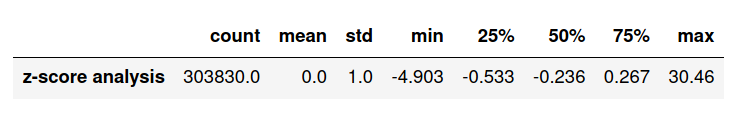
\includegraphics[scale=0.5]{images/zscore.png}
	\caption{Z score analysis for outliers}
\end{figure}

Figure 4 shows our statistics on z-score calculated, where mean of z-scores is 0 and standard deviation of z-scores is 1.0. Minimum value is -10.778 and maximum value is 40.996.
To identify the optimum value of threshold for classifying outliers we draw histogram and density plot of obtained z-score. Figure 5 and Figure 6 shows them respectively.

\begin{figure}[h]
	\centering
	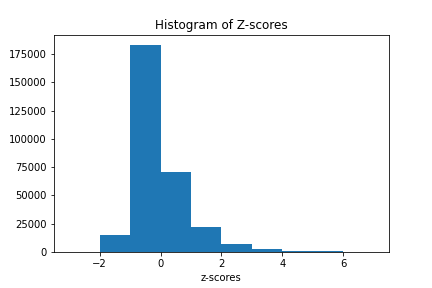
\includegraphics[scale=1]{images/zscore_histogram.png}
	\caption{Histogram of z-scores obtained from dataset}
\end{figure}

\pagebreak

\begin{figure}[h]
	\centering
	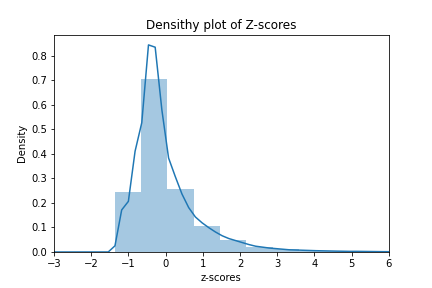
\includegraphics[scale=0.95]{images/zscore_density.png}
	\caption{Density plot of z-scores}
\end{figure}

\bigskip
From the above two plots, we observed that most of the values are near the mean of the z-scores and there is a standard deviation of +/-1. We set the the value of threshold to 4 in our analysis as there are some subsequent amount of data examples whose z-score is around +3.\\
Table 3 shows Attributes (top 10) having most number of outliers.

\begin{table}[h]
\caption{Attributes (Top 10) having most number of Outliers}
\hspace{-2cm}
\begin{tabular}{|l|c|}
\hline
\multicolumn{1}{|l|}{\textbf{Attributes Name}}                                      & \textbf{No. of Outliers} \\ \hline
\textbf{Number of Vasectomies Conducted (Public + Pvt.)} & 66 \\
\textbf{Number of Home deliveries}                       & 60 \\
\textbf{Number of home deliveries attended by Non SBA trained (trained TB/Dai)}     & 59                       \\
\textbf{Number of C-section deliveries conducted at private facilities}             & 58                       \\
\textbf{Number of Major Operations}                      & 54 \\
\textbf{Condom pieces distributed}                       & 53 \\
\textbf{Adverse Events Following Imunisation (Others)}   & 51 \\
\textbf{Number of Women Discharged under 48 hours of delivery in public facilities} & 46                       \\
\textbf{IUCD insertions done (pvt. facilities)}          & 46 \\
\textbf{Number of home deliveries attended by SBA trained (Doctor/Nurse/ANM)}       & 44                       \\ \hline
\end{tabular}
\end{table}

\pagebreak
\textbf{Boxplot on the attributes having highest and lowest number of outiler}\\

Z score results shows that every column contains decent amount of outliers, but attribute 'Number of Vasectomies Conducted (Public + Pvt.) ' contains the most outliers and attribute 'Sex Ratio at birth ( Female Live Bitrths/ Male Births *1000)' contains least amount of outliers.\\
To visualize these results we plot a boxplot corresponding these two attributes, this is shown in Figure 7.

\begin{figure}[h]
	\hspace{-1cm}
	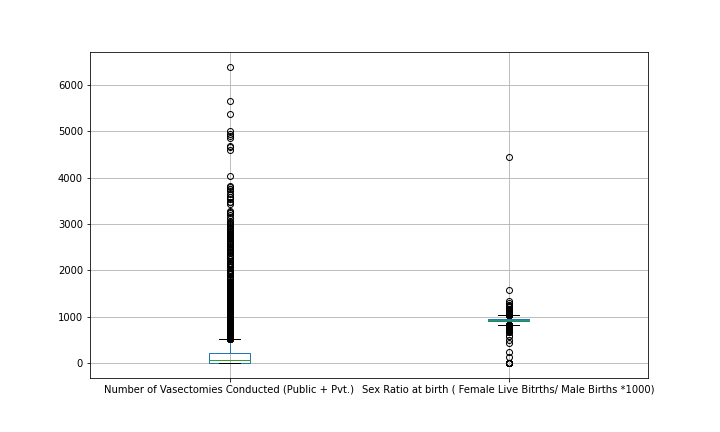
\includegraphics[scale=0.8]{images/boxplot.png}
	\caption{Boxplot on the attributes having highest and lowest number of outiler}
\end{figure}

\pagebreak
\subsubsection{Outlier Treatment}

We have identified the outliers, we need to treat them. We implemented two types of outlier techniques. From both the tests we draw different conclusions.

Attribute 'Adverse Events Following Imunisation (Others)' is on top of IQR analysis. On checking the values of this attribute we found that most of the values of this attribute is zero and because of this IQR is pointing it out as outlier. So from IQR analysis we found the attributes which has most of the values zero. Since these values are marked as outliers we can conclude these zero values are actually the missing values in the data set marked as value zero.\\
We confirmed these conclusion by training the regression model after dropping the outliers mentioned by the IQR and our prediction accuracy dropped. So we used z-score results from dropping the outliers.\\

Number of outliers in Z score test is significantly less than that of in IQR test. So we can say that the outliers pointed by the z-score test are real outlier of the dataset and these are needed to be dropped from the dataset. \\
We confirmed this conclusion by training the regression model and our accuracy improved.

\newpage

\section{Prediction}

We have three problem statements:
\begin{enumerate}
	\item Prediction of the number of child births in each district of the country.
	\item Prediction of the number of still births in each district of the country.
	\item Prediction of the number of infant deaths in each district of the country.
\end{enumerate}

Since the all three problems are of regression we applied different models of regression - Linear Regression, Ridge Regression, Lasso Regression, Elastic Net Regression and Random Forest. We have learned model for each of the problem statement separately with different indepenent and dependent variables. We have discussed them in the following three sections:

\section{CASE 1: PREDICTION OF NUMBER OF BIRTHS}

Here we predicted the number of child births in each district of India in a year from the data set available. We first learned the Linear Regression model on our data.\\

We have 47 attributes in the data set out of which we have dropped the categorical attribute - "Indicator" from our dataset. We have divided our variables into independent and dependent set as follows:\\

\textbf{Independent$\backslash$Target attribute:} 'Total Number of reported live births'\\
\textbf{Dependent attributes:} Rest 45 attributes of the dataset.\\

We used sklearn library for implementing the Linear Regression model.
\begin{file}[Linear\_Regression.py]
\#importing Linear Regression from sklearn\\
from sklearn.linear\_model import LinearRegression as LR\\

\# Creating instance of Linear Regresssion\\
lr = LR()\\

\# Fitting the model\\
lr.fit(train\_x, train\_y)
\end{file}



For Linear Regression model to work good and to give good prediction rates, the data should follow some assumptions/characterstics. These characteristics are as follows: \\ 

\textbf{Assumptions of Linear Regression}\\
Assumptions made while applying the Linear Regression model are:
\begin{itemize}
	\item \textbf{Linear relationship:} Relationship between response and feature variables should be linear.
	\item \textbf{Little or no multi-collinearity:} It is assumed that there is little or no multicollinearity in the data. Multicollinearity occurs when the features (or independent variables) are not independent from each other.
	\item \textbf{Little or no auto-correlation:} Another assumption is that there is little or no autocorrelation in the data. Autocorrelation occurs when the residual errors are not independent from each other. 
	\item \textbf{Homoscedasticity:} Homoscedasticity describes a situation in which the error term (that is, the “noise” or random disturbance in the relationship between the independent variables and the dependent variable) is the same across all values of the independent variables. 
	\item \textbf{Normality:} The errors are generated from a Normal distribution (of unknown mean and variance, which can be estimated from the data).
\end{itemize}

After learning the model, to check whether the accuracy of the model can be further improved or not, we need to verify whether all the assumptions of linear regression about the data set holds true. If some assumption do not holds true then we need to transform our data set. 

\subsection{Interpreting Regression Coefficients for Linear Relationships}

\begin{figure}[h]
\centering
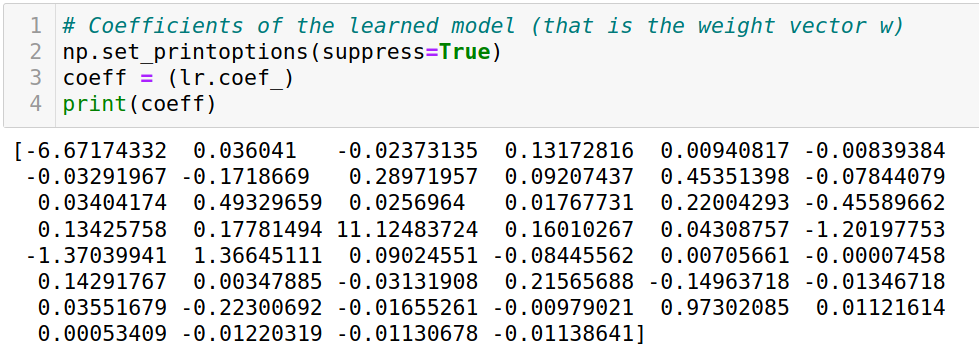
\includegraphics[scale=.4]{images/coefficients.png}
\caption{Coefficients learned by the model}
\end{figure}

The sign of a regression coefficient tells you whether there is a positive or negative correlation between each independent variable the dependent variable. A positive coefficient indicates that as the value of the independent variable increases, the mean of the dependent variable also tends to increase. A negative coefficient suggests that as the independent variable increases, the dependent variable tends to decrease.\\

The coefficient value signifies how much the mean of the dependent variable changes given a one-unit shift in the independent variable while holding other variables in the model constant. This property of holding the other variables constant is crucial because it allows you to assess the effect of each variable in isolation from the others. Following figure shows the values of the coefficients learned by the model.



\pagebreak
\subsection{Coefficient Plot}

\begin{figure}[h]
\centering
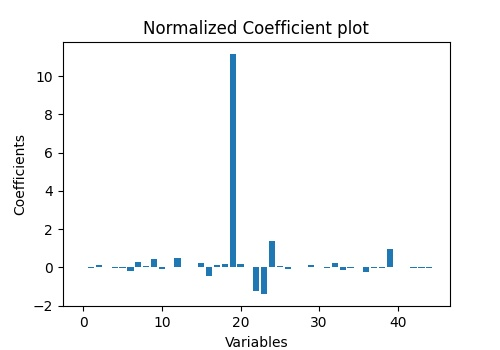
\includegraphics[scale=1]{images/coefficient_plot.jpg}
\caption{Normalized Coefficient plot}
\end{figure}

\medskip
Coefficient plot tells us that our target variable highly depends on 1 attribute and it is positve correlated. Plot shows that coefficient values of 40 attributes is very less, and only 5 attributes majorly contribute to our model's prediction. These attributes are: 

\vspace{10pt}

\begin{figure}[h]
\centering
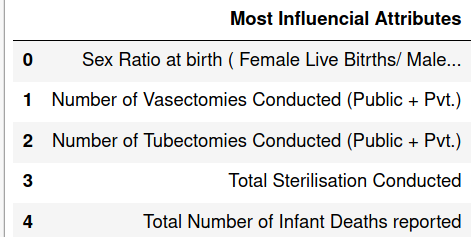
\includegraphics[scale=.5]{images/birthattributes.png}
\caption{Attributes that influenced the model most}
\end{figure}

Target attribute is positively correlated with the attributes - Sex Ratio at birth, Total Sterilisation Conducted, Total Number of Infant Deaths reported and is negatively correlated with attributes - Number of Vasectomies Conducted and Number of Tubectomies Conducted. This makes sense too as Vasectomies and Tubectomies makes humans infertile and hence will reduce the number of child births.	

\pagebreak
\subsection{Residual vs Fitted}
Residuals are the difference between the observed values and the fitted values. We need to plot the residuals, check their random nature, variance, and distribution for evaluating the model quality. This is the visual analytics needed for goodness-of-fit estimation of a linear model.

If the plot of residual vs fitted do not show any pattern then ideally it suggests linearity in the data set. Since the figure do not show any pattern so it satisfies linearity.
\begin{figure}[h]
\centering
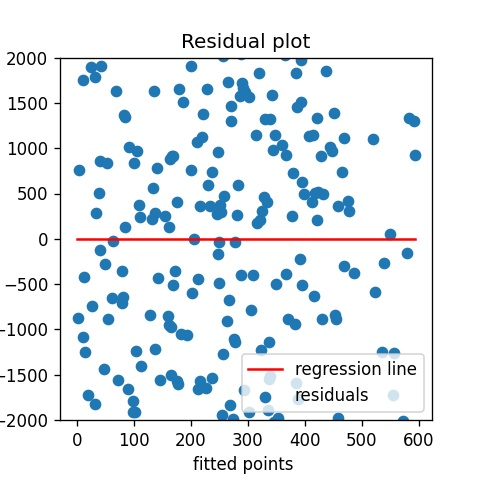
\includegraphics[scale=.8]{images/residual-plot.jpg}
\caption{Residual Plot}
\end{figure}


 The points in a residual plot are randomly dispersed around the horizontal axis and they are distributed uniformly randomly around the zero x-axes and do not form specific clusters. Hence a linear regression model is appropriate for the data.\\
 When we plot the fitted response values (as per the model) vs. the residuals, we clearly observe that the variance of the residuals remains constant with response variable magnitude. Therefore, the problem respect homoscedasticity. 

\pagebreak
\subsection{Normality Test}
To check the assumption of normality of the data generating process, we  plot the histogram and the Q-Q plot of the normalized residuals.

\begin{figure}[h]
\centering
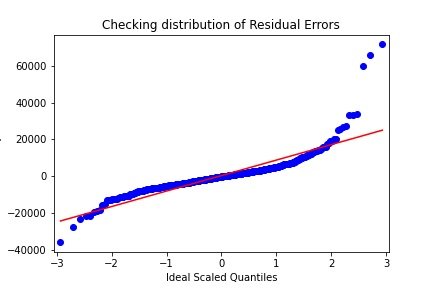
\includegraphics[scale=.75]{images/residual-qqplot.jpg}
\caption{QQ Plot for residuals}
\end{figure}

\begin{figure}[h]
\centering
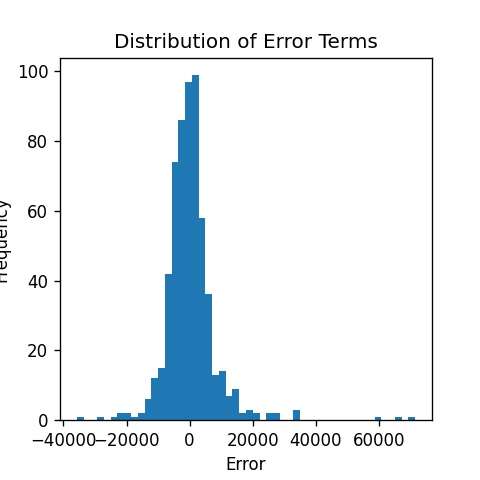
\includegraphics[scale=.8]{images/residual-histogram.jpg}
\caption{Histograms for residuals}
\end{figure}

Since the QQ plot is almost linear and fits accross the regression line and histogram plot follows normal distribution, our data set follows normality.

\pagebreak
\subsection{Evaluation of Model}

We evaluated the performance of our model from the following measures:
\begin{itemize}
	\item \textbf{RMSE:} MSE is calculated by the sum of square of prediction error which is real output minus predicted output and then divide by the number of data points. It gives you an absolute number on how much your predicted results deviate from the actual number. Root Mean Square Error(RMSE) is the square root of MSE. 
	\item \textbf{MAE:} MAE is taking the sum of absolute value of error.  MSE gives larger penalisation to big prediction error by square it while MAE treats all errors the same.
	\item \textbf{R Square (Coefficient of Determination):} R Square measures how much of variability in dependent variable can be explained by the model. It is square of Correlation Coefficient(R) and that is why it is called R Square.
\end{itemize}

Error of the linear regression model for above mentioned measures are shown in the Table 4 below.

\begin{table}[h]
\caption{Results of Linear regression model for Child Births }
\vspace{10pt}
\centering
\begin{tabular}{|l|l|}
\hline
\textbf{Measure }                        & \textbf{Error }           \\ \hline
Training Mean Absolute Error    & 2828.6132176902  \\
Test Mean Absolute Error        & 5109.2537316244  \\
Training Root Mean Square Error & 5362.25745574993 \\
Testing Root Mean Square Error  & 8402.35904407914 \\
Training Accuracy(R-square)     & 95.7276759961367 \\
Testing Accuracy(R-square)      & 93.3642138572999 \\ \hline
\end{tabular}
\end{table}

So with Linear Regression we are getting 93\% prediction accuracy, which is quite good. Since Random Forest gives better results most of the time as compared to linear regression, we learned that model too. 

\section{Random Forest Model for Predicting Births}

\begin{file}[Random\_Forest.py]
from sklearn.ensemble import RandomForestRegressor

\medskip

\# create object of Random Forest\\
regressor = RandomForestRegressor(n\_estimators = 25,random\_state = 0)

\medskip
\# fit the regressor with x and y data\\
regressor.fit(train\_x, train\_y)

\medskip
\# predicting for train and test set\\
train\_predict = regressor.predict(train\_x)\\
test\_predict = regressor.predict(test\_x)
\end{file}

\pagebreak
Figure 14 shows the plot of actual target values vs the predicted values by the model.

\begin{figure}[h]
\hspace{-3.2cm}
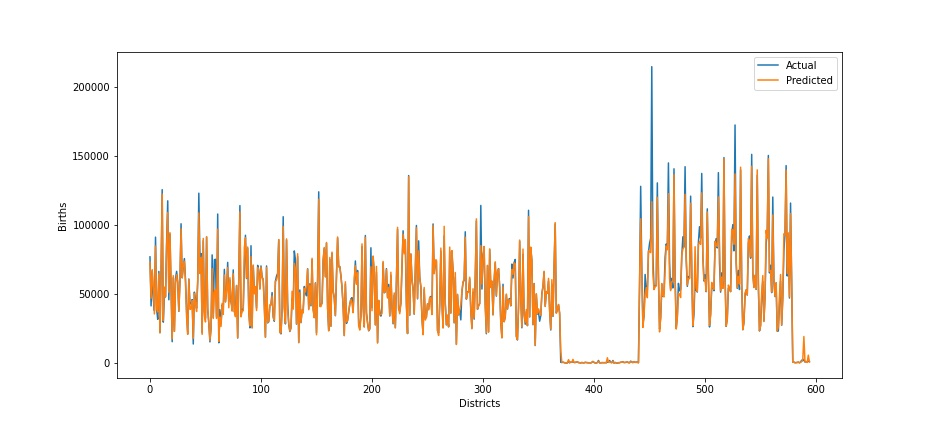
\includegraphics[scale=.7]{images/RandomForestLiveBirth.jpg}
\caption{Actual vs Predicted plot for target variable}
\end{figure}

Table 5 shows the name of the features/attributes on which our target attribute is highly dependent.

\begin{table}[!h]
\centering
\caption{}
\vspace{5pt}
\begin{tabular}{|l|}
\hline
\textbf{Important Features for Random Forest Model}          \\ \hline
Number of fully immunized children (9-11 months)                       \\
Number of pregnant women received 3 ANC check ups                      \\
Number of Infants given BCG                                            \\
Total number of pregnant women Registered for ANC                      \\
Number of Infants given OPV 0 (Birth Dose)                             \\
Deliveries Conducted at Public Institutions                            \\
TT2 or Booster given to Pregnant women (numbers)                       \\
Number of Infants given Measles                                        \\
Number of home deliveries attended by Non SBA trained (trained TB/Dai) \\
Number of Infants given DPT1             \\ \hline
\end{tabular}
\end{table}

\pagebreak

\begin{table}[h]
\centering
\caption{Results of Random Forest model for Child Births}
\vspace{5pt}
\begin{tabular}{|l|l|}
\hline
\textbf{Measure}                & \textbf{Error}   \\ \hline
Training Mean Absolute Error    & 574.652419301165 \\
Test Mean Absolute Error        & 2229.61431932773 \\
Training Root Mean Square Error & 1564.56984390149 \\
Testing Root Mean Square Error  & 5916.33023171844 \\
Training Accuracy(R-square)     & 99.6362870467858 \\
Testing Accuracy(R-square)      & 96.7100088929496 \\ \hline
\end{tabular}
\end{table}

Table 6 shows the results of evaluation measures applied on the random forest model learned. Model is having 96\% prediction rate, this is 3\% more than the linear regression.\\

\pagebreak
\section{CASE 2: PREDICTION OF NUMBER OF STILL-BIRTHS}

Here we predicted the number of still births in each district of India in a year from the data set available. The Linear Regression gives an accuracy of 92\% whereas Random Forest gives an accuracy of 98\%.\\ 


We have 47 attributes in the data set out of which we have dropped the categorical attribute - "Indicator" from our dataset. We have divided our variables into independent and dependent set as follows:\\

\textbf{Independent$\backslash$Target attribute:} 'Total Number of reported Still Births'\\
\textbf{Dependent attributes:} Rest 45 attributes of the dataset.\\
\subsection{Linear Regression}

The Linear Regression model used is same as the one used in CASE 1: Prediction of Number of Births.\\

Error and Accuracy of the linear regression model for the measures are shown in the Table 7 below.\\

\begin{table}[!h]
\centering
\caption{Results obtained for Still Births}
\vspace{5pt}
\begin{tabular}{|l|l|}
\hline
\textbf{Measure}                & \textbf{Error}   \\ \hline
Training Mean Absolute Error    & 1023.99261949344 \\
Test Mean Absolute Error        & 2390.04152966319 \\
Training Root Mean Square Error & 2235.31247540752 \\
Testing Root Mean Square Error  & 4821.80489352115 \\
Training Accuracy(R-square)     & 88.124395801068  \\
Testing Accuracy(R-square)      & 92.4555099954537	\\ \hline
\end{tabular}
\end{table}

So with Linear Regression we are getting 92\% prediction accuracy, which is quite good.\\


The most Influential Attributes as per the Linear Regression model for the predictions of Still Births are mentioned in the Table 8 below.\\

\begin{table}[!h]
\centering
\caption{}
\vspace{5pt}
\begin{tabular}{|l|}
\hline
\textbf{Most Influencial Attributes}              \\ \hline
Number of Home deliveries                         \\
Number of home deliveries attended by SBA trai... \\
Number of home deliveries attended by Non SBA ... \\
Institutional deliveries (Public Insts.+Pvt. I... \\
Total reported deliveries                         \\
Sex Ratio at birth ( Female Live Births/ Male... \\
Number of Vasectomies Conducted (Public + Pvt.)   \\
Number of Tubectomies Conducted (Public + Pvt.)   \\
Total Sterilisation Conducted                    \\ \hline
\end{tabular}
\end{table}
\\
Target attribute is co-related related to the attributes representing various types of deliveries conducted. The most influential attribute is Number of Home deliveries. This make sense too since there are complications attached with Home deliveries. It is clearly seen from the table that Still Births depend mostly on the no of Deliveries conducted, and also makes sense too. The other attributes : Sex Ratio at birth, Number of Vasectomies/ Tubectomies, Total Sterlisation Conducted are also highly related to the prediction of Still Births.\\

Since Random Forest gives better results most of the time as compared to linear regression, we learned that model too.\\
\newpage
\subsection{Random Forest}
Figure 15 shows the plot of actual target values vs the predicted values by the model.\\

\begin{figure}[h]
\hspace{-3.2cm}
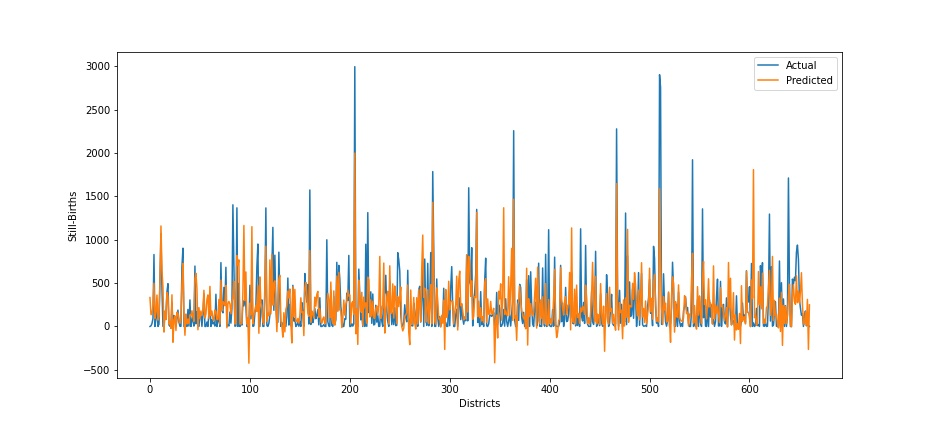
\includegraphics[scale=.7]{images/RandomForestStillBirth.jpg}
\caption{Actual vs Predicted plot for target variable}
\end{figure}

Table 9 shows the name of the features/attributes on which our target attribute is highly dependent.\\
\begin{table}[!h]
\centering
\caption{}
\vspace{5pt}
\begin{tabular}{|l|}
\hline
\textbf{Important Features for Random Forest Model}          \\ \hline
Number of Infants given BCG                                      \\
Number of Newborns having weight less than 2.5 Kg                 \\
Total reported deliveries                                        \\
TT2 or Booster given to Pregnant women (numbers)                 \\                         
Condom pieces distributed                                        \\
Institutional deliveries (Public Insts.+Pvt. Insts.)          \\
Total Number of reported live births                              \\
Total number of pregnant women Registered for ANC                   \\
Number of Pregnant women registered within first trimester                                                          \\
Number of Minor Operations             \\ 
\hline
\end{tabular}
\end{table}
\begin{table}[h]
\centering
\caption{Results of Random Forest model for Still Births}
\vspace{5pt}
\begin{tabular}{|l|l|}
\hline
\textbf{Measure}                & \textbf{Error}   \\ \hline
Training Mean Absolute Error    & 89.88106998654105 \\
Test Mean Absolute Error        & 541.9993948562783 \\
Training Root Mean Square Error & 396.0021534095236 \\
Testing Root Mean Square Error  & 2139.573840681855 \\
Training Accuracy(R-square)     & 99.62728718459579 \\
Testing Accuracy(R-square)      & 98.51452557349563 \\ \hline
\end{tabular}
\end{table}

Table 10 shows the results of evaluation measures applied on the random forest model learned. Model is having 98\% prediction rate, this is 6\% more than the linear regression.\\




\newpage
\section{CASE 3: PREDICTION OF NUMBER OF INFANT-DEATHS}
Here we predicted the number of infant deaths in each district of India in a year from the data set available.\\
The Prediction accuracy using Linear Regression is 49\% and it increases to 69\% for Random Forest. The attributes in the data available on HMIS portal is good for prediction for Births and Still Births but is not very useful in predicting the no of infant deaths.\\


We have 47 attributes in the data set out of which we have dropped the categorical attribute - "Indicator" from our dataset. We have divided our variables into independent and dependent set as follows:\\

\textbf{Independent$\backslash$Target attribute:} 'Total Number of reported Infant Deaths'\\
\textbf{Dependent attributes:} Rest 45 attributes of the dataset.\\



\subsection{Linear Regression}
Figure 16 below shows the Actual vs Predicted plot for target variable using Linear Regression.
\begin{figure}[h]
\hspace{-3.2cm}
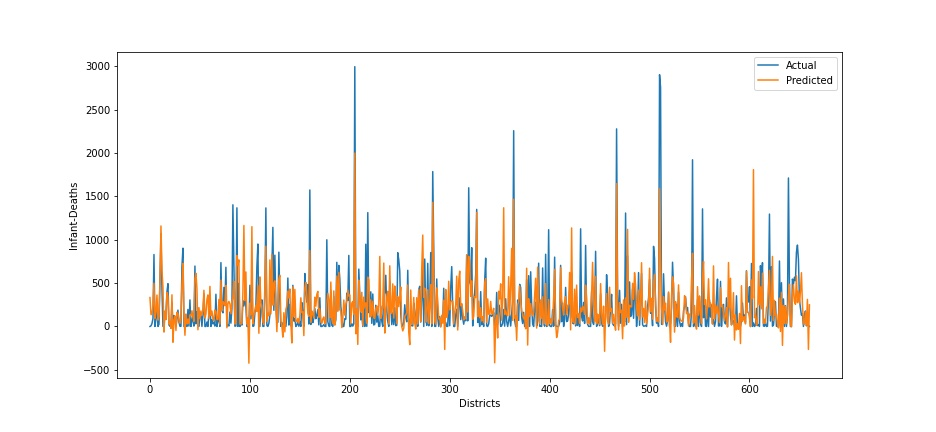
\includegraphics[scale=.7]{images/RandomForestInfantDeaths.jpg}
\caption{Actual vs Predicted plot for target variable for Linear Regression}
\end{figure}

Error and Accuracy of Linear Regression for prediction of Infant deaths is shown in the below table 11. 

\begin{table}[h]
\centering
\caption{Results of Infant Deaths by Linear Regression}
\vspace{5pt}
\begin{tabular}{|l|l|}
\hline
\textbf{Measure}                & \textbf{Error}     \\ \hline
Training Mean Absolute Error    & 176.98444922111506 \\
Test Mean Absolute Error        & 171.44992601028855 \\
Training Root Mean Square Error & 284.300609512833   \\
Testing Root Mean Square Error  & 265.06288848278155 \\
Training Accuracy(R-square)     & 48.09697806858291  \\
Testing Accuracy(R-square)      & 49.51743097935387 \\ \hline
\end{tabular}
\end{table}
The most important features in the prediction of infant deaths using Linear Regression Model are mentioned in the figure 17.
\begin{figure}[h]
\centering
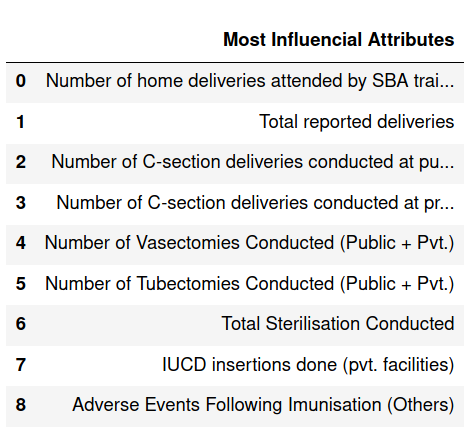
\includegraphics[scale=.5]{images/features-of-infant-death-linear-regression .png}
\caption{Important features of Infant Death Linear Regression}
\end{figure}

\subsection{Analysing Failure of Linear Regression}

For Linear Regression model to work and to give good prediction rates, the data should follow some assumptions/characteristics. The main characteristics are Normality, Homoscedasticity, Linear Relationship and Multi-collinearity. The details about these assumptions are discussed earlier in this report. We will now examine these characteristics in this case to reason about the failure of Linear Regression.

\subsubsection{Coefficient plot}
Coefficient plot tells us that out target variable is highly dependent on 2 variables and it is positive correlated to one variable while negative correlated to another variable. \\
\pagebreak
\begin{figure}[h]
\centering
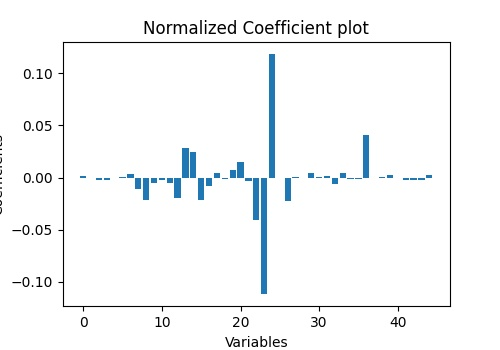
\includegraphics[scale=.99]{images/death/death-coefficient_plot.jpg}
\caption{Normalized Coefficient Plot}
\end{figure}

Plot shows coefficients values of 36 attributes is very less and only 9 attributes majorly contribute to our models prediction. These attributes are:\\
\begin{figure}[h]
\centering
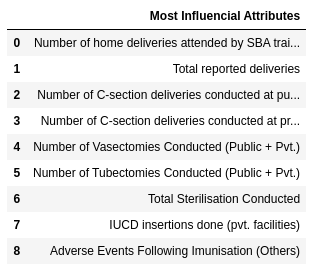
\includegraphics[scale=.7]{images/death/attr_deathlinear.png}
\caption{Attributes that influence the model most}
\end{figure}

\subsubsection{Residual plot}
Residuals are the difference between the observed values and the fitted values. We need to plot the residuals, check their random nature, variance, and distribution for evaluating the model quality. This is the visual analytics needed for goodness-of-fit estimation of a linear model.\\

If the plot of residual vs fitted do not show any pattern then ideally it suggests linearity in the data set. Since the figure do not show any pattern so it satisfies linearity.\\
\begin{figure}[h]
\centering
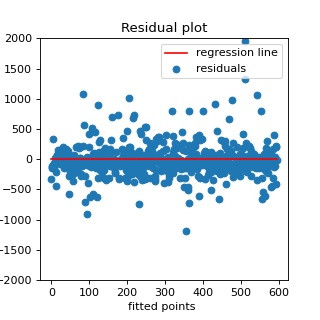
\includegraphics[scale=.9]{images/death/death-residual-plot.jpg}
\caption{Residual Plot}
\end{figure}

 When we plot the fitted response values (as per the model) vs. the residuals, we clearly observe that the variance of the residuals remains constant with response variable magnitude. Therefore, the problem respect homoscedasticity. But residuals are not distributed uniformly, they are pretty symmetrically distributed, tender to cluster towards the middle of the plot.\\
\subsubsection{Normality Test}
To check the assumption of normality of the data generating process, we  plot the histogram and the Q-Q plot of the normalized residuals.\\
\pagebreak
\begin{figure}[h]
\centering
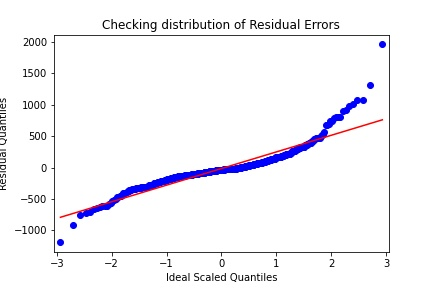
\includegraphics[scale=.80]{images/death/death-residual-qqplot.jpg}
\caption{QQ Plot for residuals}
\end{figure}

\begin{figure}[h]
\centering
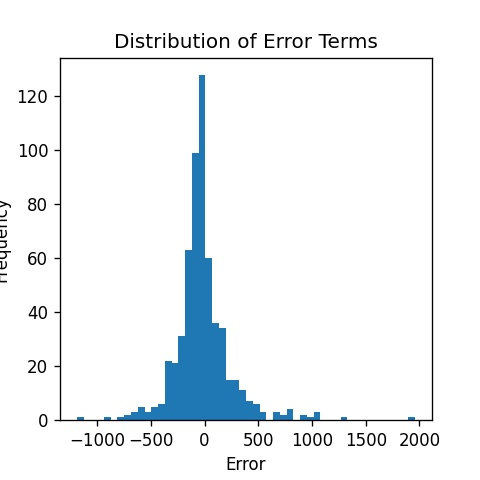
\includegraphics[scale=.7]{images/death/death-residual-histogram.jpg}
\caption{Histograms for residuals}
\end{figure}

From Histogram and QQ-plot of residuals we can say that data-set in normal for target variable-infant deaths.\\

Since data satisfies condition of normality, homoscedasticity, Linear relationship. Last thing left is check for Multicolinearity. Variance Inflation Factor test is best suited for it. if VIFk=1, variable k is not correlated to any other independent variable. As a rule of thumb, multicolinearity is a potential problem whn VIFk is greater than 4; and a serious problem when it is greater than 10.\\

\subsubsection{VIF}
After running the VIF test, it was seen that 27 out of 46 attributes have VIF greater than 10, it shows that our data suffers from heavy multicollinearity.\\

\begin{figure}[h]
\hspace{-2.5cm}
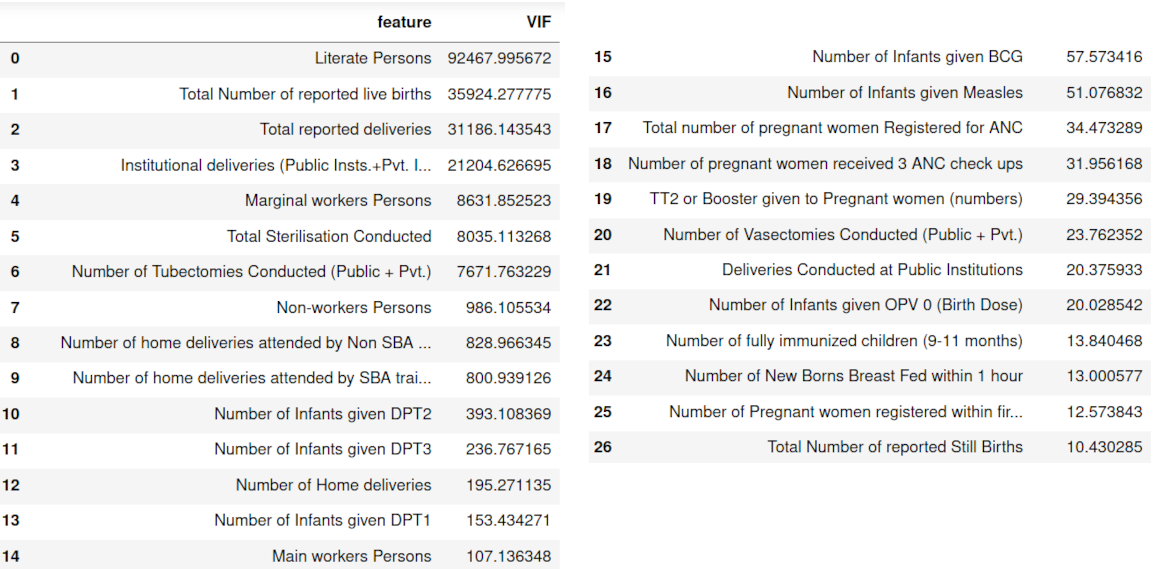
\includegraphics[scale=.45]{images/vif1.png}
\caption{VIF1}
\end{figure}

The model was trained again after dropping the attributes having VIF greater than 10, the accuracy was dropped to 37\%. The VIF was then calculated for the remaining attributes.\\

\begin{figure}[h]
\centering
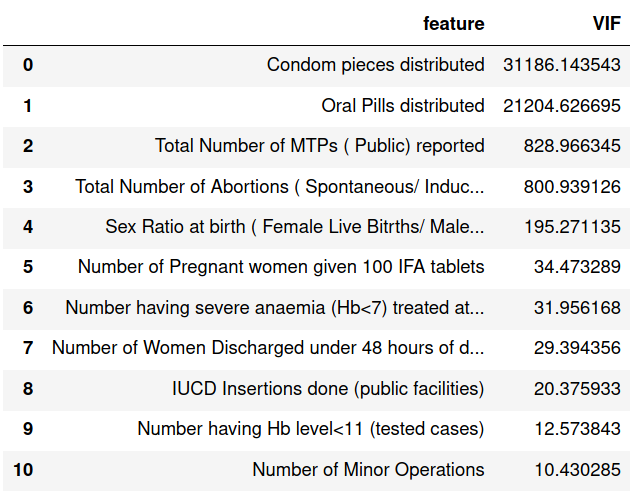
\includegraphics[scale=.35]{images/vif2.png}
\caption{VIF2}
\end{figure}

Since 11 out of the remaining 19 attributes are having VIF values greater than 10 in the remaining data-sets. We can conclude that attributes of the data-set is highly correlated with each other and accuracy of regression model will always suffer. Let us apply Random Forest on this problem.\\
\subsection{Random Forest}

Figure 25 shows that actual target values vs the predicted values by the model.\\
\begin{figure}[h]
\hspace{-3.2cm}
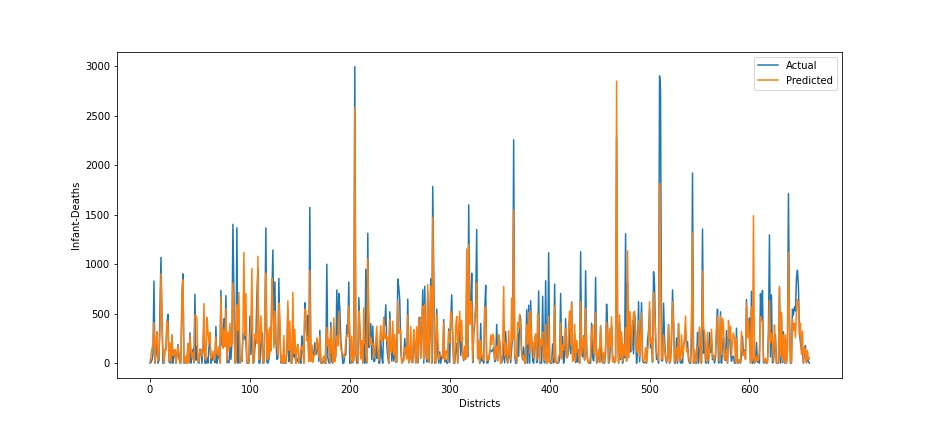
\includegraphics[scale=.7]{images/RandomForestInfantDeathrandom.jpg}
\caption{Actual vs Predicted plot for target variable for Random Forest}
\end{figure}

Table 12 below shows the results of evaluation measures applied on the Random Forest model learned. Model is having 70\% accuracy which is greater than linear regression model by 21\%. 
\begin{table}[!h]
\centering
\caption{Results obtained for Infant-Deaths by Random Forest}
\vspace{5pt}
\begin{tabular}{|l|l|}
\hline
\textbf{Measure}                & \textbf{Error}   \\ \hline
TTraining Mean Absolute Error    & 44.47679676985195  \\
Test Mean Absolute Error        & 113.2001815431165  \\
Training Root Mean Square Error & 87.23965230976026  \\
Testing Root Mean Square Error  & 201.14927401387413 \\
Training Accuracy(R-square)     & 95.12455070018713  \\
Testing Accuracy(R-square)      & 70.56988968985102	\\ \hline
\end{tabular}
\end{table}

Table 13 below shows the name of attributes/ features on which our target attribute is highly dependent.\\

\begin{table}[h]
\centering
\caption{Random Forest Important Features}
\vspace{5pt}
\begin{tabular}{|l|}
\hline
\textbf{Most Influencial Attributes}                                   \\ \hline
Total Number of reported Still Births                                  \\
Total Number of Abortions ( Spontaneous/ Induced) Reported             \\
Total Sterilisation Conducted                                          \\
Total Number of reported live births                                   \\
Number of C-section deliveries conducted at public facilities          \\
Oral Pills distributed                                                 \\
Number of Major Operations                                             \\
Number of home deliveries attended by Non SBA trained (trained TB/Dai) \\
IUCD Insertions done (public facilities)                               \\
Marginal workers Persons           \\ \hline                                   
\end{tabular}
\end{table}

\section{Results}
The training and testing score using different Machine Learning Techniques:


\begin{table}[h]
    \centering
    \begin{tabular}{||c c c c||}

\hline
Model Name&Problem Statement&Training Score&Testing Score  \\[1ex]
 \hline \hline
Linear Regression&Child Births&0.957267 &0.933956 \\[1ex]
 \hline
Random Forest&Child Births&0.993489&0.960923\\[1ex]
\hline
Linear Regression&Still Births&0.881243&0.924555\\[1ex]
\hline
Random Forest&Still Births&0.996272&0.985145\\[1ex]
\hline
Linear Regression&Infant Deaths&0.480969&0.495174\\[1ex]
\hline
Random Forest&Infant Deaths&0.9512345&0.705698\\[1ex]
\hline

\end{tabular}
    \caption{Prediction Accuracy}

\end{table}

The Random Forest Regressor Model performs the best in all the three problem statements.


\section{Discussion}
In this project we have seen that Random forest works very well in the prediction of no of child births and still births against linear regression. The main reasons can be understood from the below points:\\
Decision Trees are great for obtaining non-linear relationships between input features and the target variable.\\
Random Forest is an ensemble of decision tress. This is to say that many trees, constructed in a certain "random" way form a Random forest.\\
The averaging makes a Random Forest better than a single decision tree hence improves its accuracy and reduces over-fitting.\\
A prediction from the Random Forest Regressor is an average of the predictions produced by the trees in the forest.\\
\section{Future Directions}
There are several health schemes run by Government but the data is not available in the public domain for the most of the schemes. If in future we come across any data-sets that might be helpful further in our predictions we plan to improve prediction for the infant deaths and also for the overall project.

\section{Important Links and References}

\noindent\begin{enumerate}[leftmargin=0cm,itemindent=.5cm,labelwidth=\itemindent,labelsep=0cm,align=left]
\item HMIS Database:\url{https://www.nrhm-mis.nic.in/hmisreports/frmstandard_reports.aspx}
\item Census Data 2001:\url{https://censusindia.gov.in/DigitalLibrary/TablesSeries2001.aspx}
\item Census Data 2011:\url{https://censusindia.gov.in/2011census/population_enumeration.html}
\item GitHub Link for the project: \url{https://github.com/kuldeeps5/DataMiningFinalProject}
\item Implementation of Lasso and Ridge Regression: \\\url{https://analyticsindiamag.com/hands-on-implementation-of-lasso-and-ridge-regression/}
\item Random Forest Regression:\\ \url{https://www.geeksforgeeks.org/random-forest-regression-in-python/}
\end{enumerate}




\end{document}
